\begin{section}{Modelo Entidad Relaci\'on}

\begin{subsection}{Diagrama de entidad relaci\'on}

%diagramita del DER
\begin{figure}[H]
        \centering
        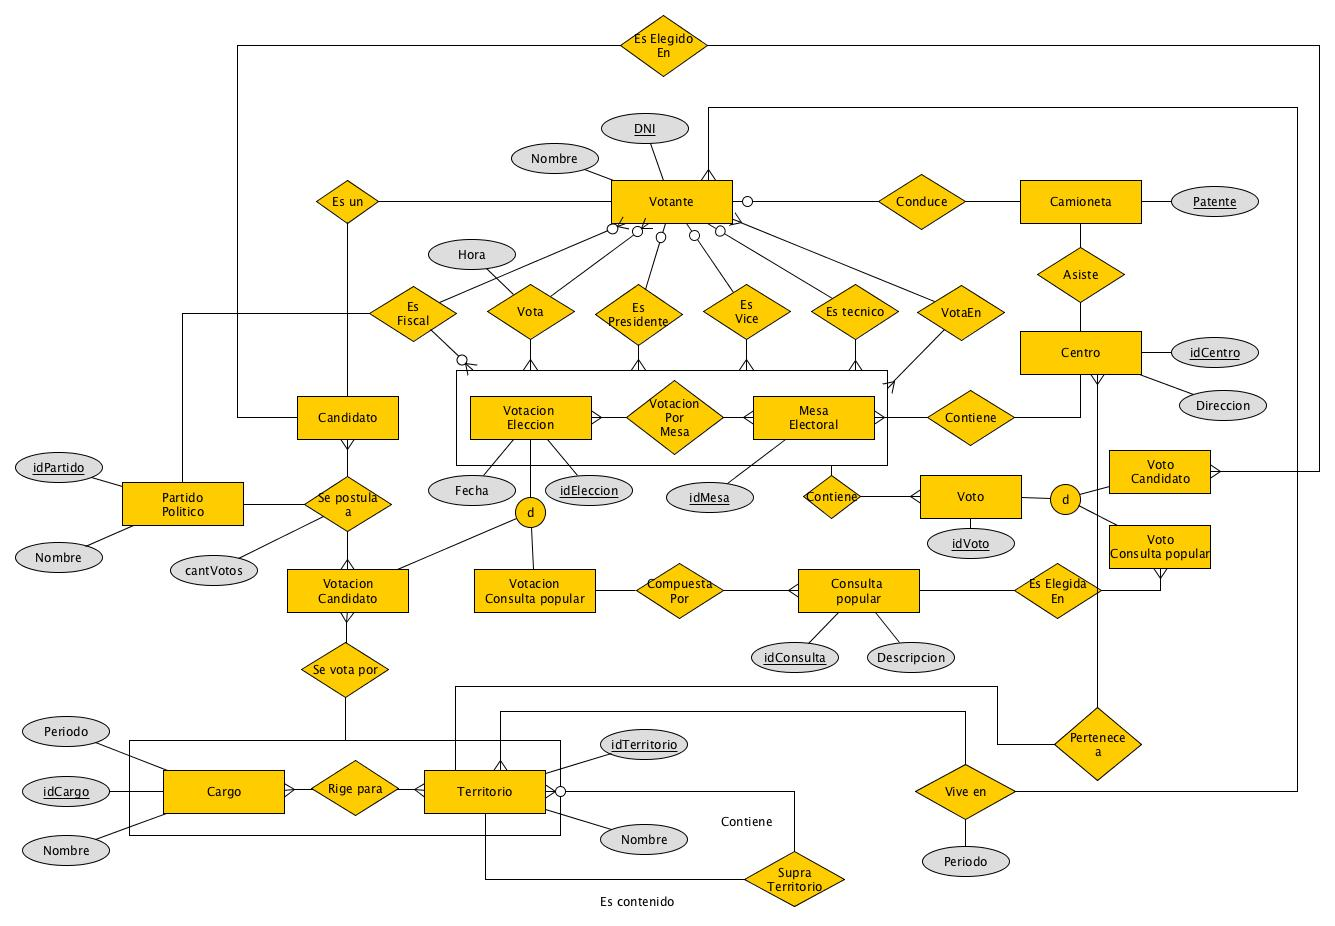
\includegraphics[angle=270,scale=0.4]{der.jpg}
\end{figure}

\end{subsection}

\begin{subsection}{Aclaraciones en lenguaje natural}

\begin{itemize}

\item La cantidad de los votos de una elecci\'on tiene que ser igual a la sumatoria de los votos obtenidos por todos los candidatos en esa elecci\'on.

\item La cantidad de votos debe ser menor o igual a la cantidad de ciudadanos en la sumatoria de los padrones de las mesas de esa elecci\'on.

\item (*) Se deben cumplir que existan los cargos de ``presidente", ``Vicepresidente'' y ``t\'ecico" por cada mesa en cada elecci\'on.

\item (*) Un mismpo votante no puede ocupar m\'as de un cargo por elecci\'on (Presidente, vicepresidente, t\'ecnico o fiscal).

\item Un votante solo puede votar en las elecciones que sean del territorio al cual pertenece cuando se realiza la elecci\'on o las de los supraterritorios.

\item La cantidad de votos que un candidato posee en sePostulaA debe ser igual a la sumatoria de los votos obtenidos por mesa para esa elecci\'on.

\item Los centros deben estar dentro del territorio en la cual se efectua la elecci\'on.

\item Un votante no puede votar m\'as de una vez por elecci\'on.

\item Un votante solo puede votar en la mesa en la que est\'e empadronado para la elecci\'on dentro de la relaci\'on votaEn.

\end{itemize}

\end{subsection}

\end{section}
